\documentclass[tikz,border=10pt]{standalone}
\usepackage{tikz}
\usepackage{amsmath}
\usepackage{mathrsfs}

\begin{document}
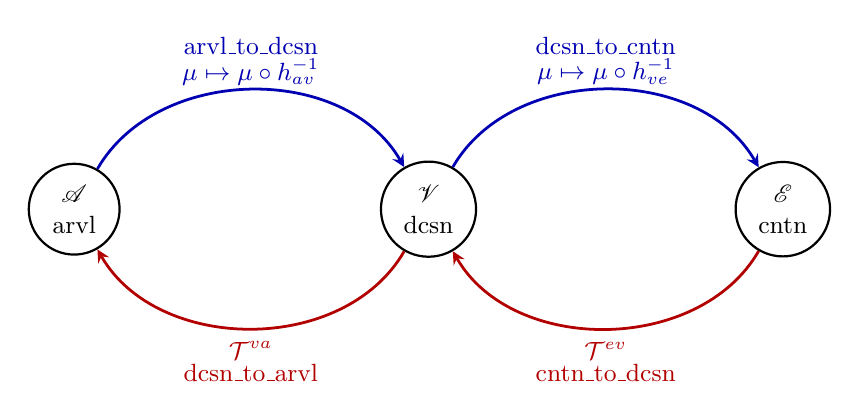
\begin{tikzpicture}[
    >=stealth,
    line width=0.8pt,
    every node/.style={font=\small},
    forwardarrow/.style={->,color=blue!70!black},
    backwardarrow/.style={<-,color=red!70!black},
    nodecircle/.style={circle,draw,minimum size=1.1cm},
]

% -- Nodes (Perches) --
\node[nodecircle, align=center] (arvl) at (0,0) {$\mathscr{A}$ \\ $\mathrm{arvl}$};
\node[nodecircle, align=center] (dcsn) at (4.5,0) {$\mathscr{V}$ \\ $\mathrm{dcsn}$ };
\node[nodecircle, align=center] (cntn) at (9,0) {$\mathscr{E}$ \\ $\mathrm{cntn}$};

% -- Forward and Backward Arrows (Curved) --
% Forward (top arcs)
\draw[->, line width=1pt, color=blue!70!black]
    (arvl) to[out=60,in=120] 
    node[above,yshift=0.9em,midway] {$\mathrm{arvl\_to\_dcsn}$}
    node[above,yshift=-0.2em,midway] {\(\mu \mapsto \mu \circ h_{av}^{-1}\)} 
    (dcsn);

\draw[->, line width=1pt, color=blue!70!black]
    (dcsn) to[out=60,in=120] 
    node[above,yshift=0.9em,midway] {$\mathrm{dcsn\_to\_cntn}$}
    node[above,yshift=-0.2em,midway] {\(\mu \mapsto \mu \circ h_{ve}^{-1}\)} 
    (cntn);

% Backward (bottom arcs)
\draw[<-, line width=1pt, color=red!70!black]
    (arvl) to[out=-60,in=-120] 
    node[below,yshift=-0.9em,midway] {$\mathrm{dcsn\_to\_arvl}$}
    node[below,yshift=-0.1em,midway] {\(\mathcal{T}^{va}\)} 
    (dcsn);

\draw[<-, line width=1pt, color=red!70!black]
    (dcsn) to[out=-60,in=-120] 
    node[below,yshift=-0.9em,midway] {$\mathrm{cntn\_to\_dcsn}$}
    node[below,yshift=-0.1em,midway] {\(\mathcal{T}^{ev}\)} 
    (cntn);

\end{tikzpicture}
\end{document}
